\section{方案实现}
为实现高保真、视角连贯且几何对齐的三维纹理生成，
本工作的核心思想是将二维生成模型\cite{podell2023sdxl, huang2025mv}中蕴含的丰富学习先验
与原生三维纹理表示\cite{xiang2025native}的固有优势相结合。
基于这一出发点，我们提出了一种多视角引导的原生三维纹理生成框架，
在保留细粒度纹理细节的同时，有效促进全局跨视角一致性与几何对齐。
本节其余部分组织如下：
第~\ref{sec:overview}~节概述整体框架；
第~\ref{sec:multview}~节介绍本文使用的多视角扩散模型；
第~\ref{sec:finetune}~节详细阐述微调原生纹理生成模型的细节；
第~\ref{sec:user}~节介绍用户界面与交互流程。

\subsection{整体框架}
\label{sec:overview}

\begin{figure}[htbp]
    \centering
    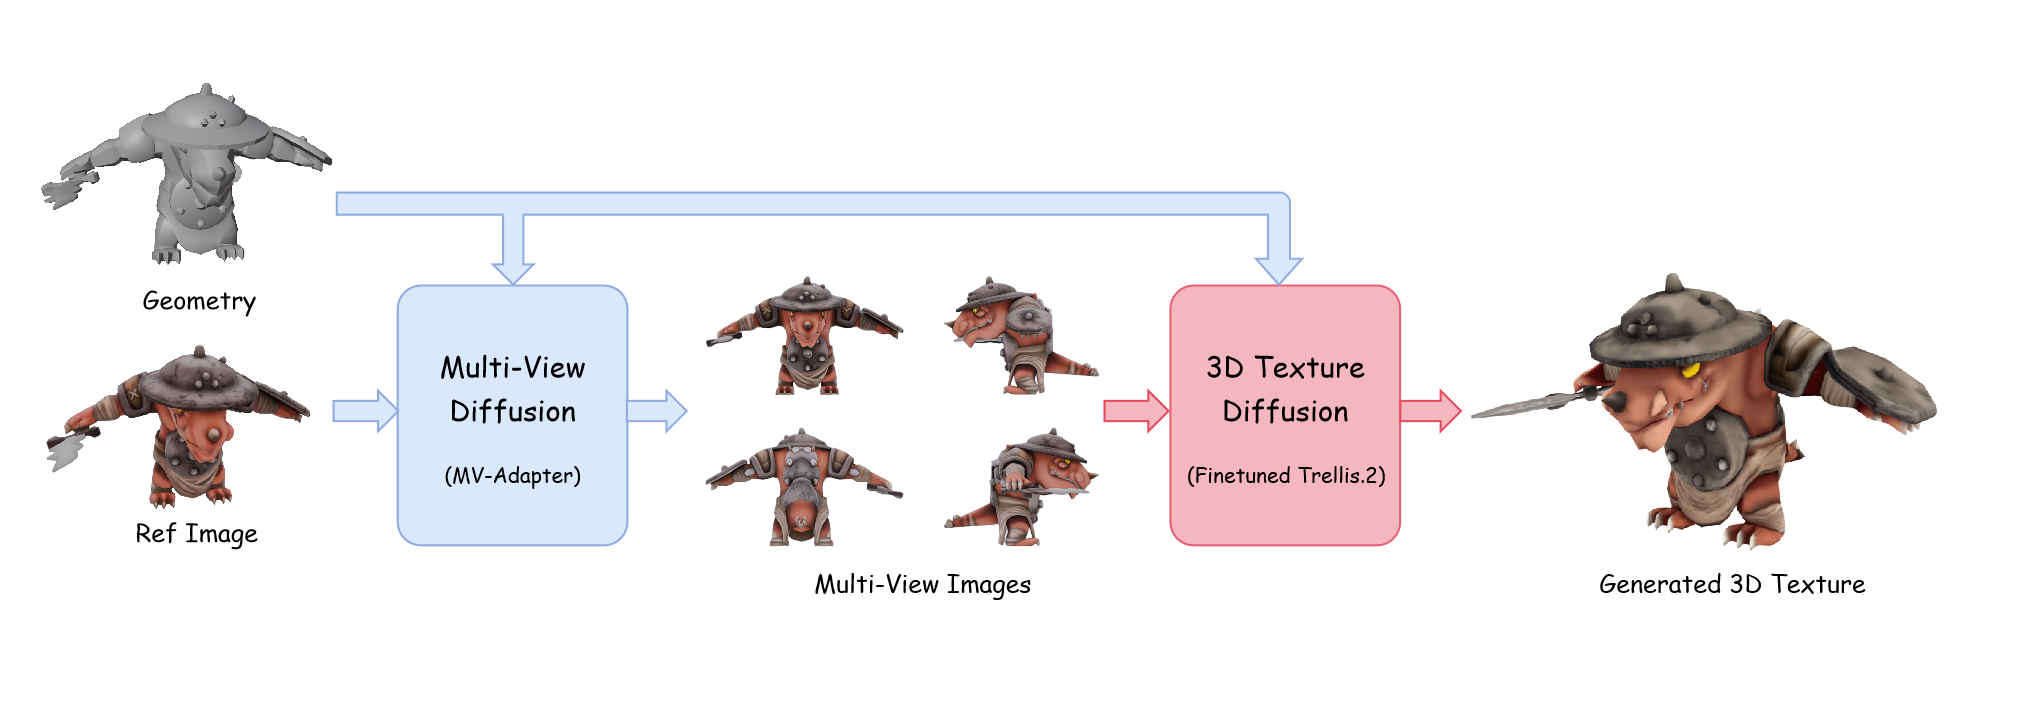
\includegraphics[width=\linewidth]{figure/final/pineline.png}
    \caption{整体框架}
    \label{fig:pipeline}
\end{figure}
本论文提出的整体框架如图~\ref{fig:pipeline}~所示。
该框架以裸网格（Input Geometry）与参考纹理图像（Reference Image）作为输入。
首先，参考图像与裸网格共同送入多视角扩散模型MV-Adapter， 
生成几何对齐的多视角纹理图像。随后，所生成的多视角图像连同原始几何信息一并输入经过微调的三维纹理扩散模型
Trellis.2\cite{xiang2025native} 三维纹理扩散模型，以多视角一致性为约束，
直接在三维空间中生成高保真纹理，最终输出完整的纹理化三维模型。

\subsection{多视图扩散模型}
\label{sec:multview}
本文采用 MV-Adapter\cite{huang2025mv} 作为多视角图像生成模块。
MV-Adapter 是一种即插即用的适配器，
在不修改预训练 SDXL 模型原始网络结构与特征空间的前提下，
通过引入解耦注意力机制与统一条件编码器，
实现几何引导与图像引导的多视角一致性生成。

在几何条件方面，MV-Adapter 对裸网格 $\mathcal{M}$ 进行多视角渲染，
得到各视角下的位置图（Position Map）与法向图（Normal Map），
并将二者拼接作为几何条件输入。
位置图提供跨视角的空间点对应关系，法向图则捕捉细粒度的几何细节，
二者共同经由轻量卷积条件编码器提取多尺度特征，
以残差形式注入 UNet 各尺度编码层，引导生成结果与网格几何精确对齐。

在图像条件方面，MV-Adapter 通过图像交叉注意力层
（Image Cross-Attention）引入参考图像的外观先验。
该层由预训练空间自注意力层复制初始化，
并与多视角注意力层共同组织为并行注意力架构：
\begin{equation}
    f^{self} = \text{SelfAttn}(f^{in}) + \text{MVAttn}(f^{in}) 
    + \text{ImgCrossAttn}(f^{in}, f^{ref}) + f^{in}
\end{equation}
其中 $f^{ref}$ 为参考图像经预训练 UNet 前向传播所缓存的中间特征。
并行结构使新增注意力层能够充分继承预训练模型的外观先验，
从而高效学习跨视角一致性与几何对应关系。

最终，模型在单次推理中同步输出 $K$ 张几何对齐的多视角图像
$\{\mathbf{I}_i\}_{i=1}^{K}$，为后续三维纹理生成提供高质量的外观约束。

\subsection{以多视图为输入的三维纹理扩散模型}
\label{sec:finetune}

\subsubsection{基线模型}

本文以 Trellis.2\cite{xiang2025native} 作为三维纹理生成的基线模型。
Trellis.2 提出了一种名为 O-Voxel 的原生三维表示，
将几何与材质属性统一编码于稀疏体素结构之中。
每个活跃体素同时存储几何特征（顶点位置、边相交标志、分割权重）
与材质特征（基础色 $c$、金属度 $m$、粗糙度 $r$、不透明度 $\alpha$），
从而实现几何与 PBR 材质的端到端原生三维生成，
无需多视角烘焙或视角相关后处理。

在表示学习方面，Trellis.2 设计了稀疏压缩 VAE（SC-VAE），
对 O-Voxel 数据进行 16 倍空间下采样，
将一个 $1024^3$ 分辨率的完整纹理资产压缩至约 9.6K 个潜变量 token，
为高分辨率三维生成提供紧凑的潜在空间基础。

在生成流程方面，Trellis.2 采用三阶段级联生成策略：
（1）稀疏结构生成，预测稀疏体素网格的占据布局；
（2）几何生成，在活跃体素内预测几何潜变量；
（3）材质生成，在几何结构约束下合成 PBR 材质潜变量。
其中，材质生成阶段采用稀疏 DiT 模型，
以输入图像特征与几何潜变量为联合条件，
直接在原生三维潜变量空间中预测材质分布，
确保材质与几何在任意拓扑结构下的空间对齐。

在纹理迁移场景下，给定目标网格，
可跳过前两个阶段，
仅激活材质生成阶段对网格进行纹理合成。
然而，原始 Trellis.2 以单张图像作为条件输入，
仅能感知参考图像中可见区域的外观信息，
对遮挡区域的纹理推断能力有限，
导致背面等不可见区域的生成质量明显下降。
为此，本文对材质生成阶段进行微调，
以多视角图像替代单张图像作为条件输入，
在保留原生三维生成优势的同时，
有效提升全局纹理的一致性与细节保真度。

\subsubsection{多视角条件微调}
原始 Trellis.2 的材质生成阶段以单张图像为条件，
通过 DINOv3 特征提取器\cite{simeoni2025dinov3}编码图像特征，
联合几何潜变量驱动稀疏 DiT 在三维潜变量空间中预测材质分布。
为使模型感知完整的全局外观信息，
本文将条件输入由单张图像扩展为多视角图像集合，
并对材质生成阶段进行轻量化微调。

在微调阶段，我们基于 TRELLIS.2 中材质生成阶段的 Sparse DiT 模型，对其 512 分辨率配置进行微调。
具体而言，仅在注意力模块的投影矩阵中引入低秩更新分支，其余参数均保持冻结，
从而在不破坏预训练生成先验的前提下实现轻量化微调。
对于任一线性层权重 $W \in \mathbb{R}^{d \times d}$，LoRA 将其参数化为：
\begin{equation}
W' = W + \Delta W,
\end{equation}
其中低秩增量定义为：
\begin{equation}
\Delta W = \frac{\alpha}{r} BA,
\end{equation}
其中 $A \in \mathbb{R}^{r \times d}$，$B \in \mathbb{R}^{d \times r}$，$r$ 表示低秩维度，$\alpha$ 为缩放系数。
在本工作中，我们设置 $r=16$，$\alpha=32$，对应缩放比例 $\alpha / r = 2.0$，
并在 LoRA 分支中引入 dropout（rate = 0.05）以增强正则化能力。
为保证微调初始阶段模型行为与预训练模型严格一致，我们采用如下初始化策略：
矩阵 $A$ 采用 Kaiming 均匀分布初始化，矩阵 $B$ 初始化为零矩阵。
因此在训练开始时满足：
\begin{equation}
\Delta W = BA = 0,
\end{equation}
从而保证模型在初始前向传播时等价于原始预训练模型，
仅在训练过程中逐步学习低秩增量以适应多视角条件建模任务。
该设计在保留预训练先验的同时，实现了对多视角条件的高效适配。

在条件编码上，本文将 $K=4$ 张正交视角图像按照 $2 \times 2$ 网格进行拼接，
构成一张分辨率为 $1024 \times 1024$ 的大图，
并将其作为整体输入送入 DINOv3 特征提取器\cite{simeoni2025dinov3}进行前向编码。
该设计使模型能够在单次前向传播中同时建模多视角外观信息，从而显著提升跨视角一致性建模效率。
所得全局特征被用作多视角外观条件，并通过交叉注意力机制注入 DiT 主干网络。

在训练阶段，采用无分类器引导（Classifier-Free Guidance, CFG）\cite{ho2022classifier}，
以概率 $p = 0.1$ 随机丢弃图像条件，从而学习无条件生成先验。
在推理阶段，通过调节 guidance scale 在条件预测与无条件预测之间进行加权融合，
以提升生成质量与稳定性。
优化过程中采用 AdamW 优化器\cite{loshchilov2017decoupled}，
学习率设置为 $3 \times 10^{-4}$，权重衰减为 0.01，
并使用 bfloat16 混合精度训练，每张 GPU 的批大小为 4。
训练在 4 块 NVIDIA RTX 5090 GPU 上进行，
总训练步数为 $10^5$，共计约 50 小时。

\subsubsection{训练数据}

本文基于 Texverse 数据集\cite{zhang2025texverse}构建训练数据，
从中初步收集约 4 万个三维模型资源。
首先，使用 Blender 对每个模型进行渲染，
生成其正面视角图像，用于初步质量检查与筛选。
为保证数据质量，我们进一步引入视觉语言模型
GLM-4.6V-Flash，
对渲染结果进行自动筛选，
筛选阶段采用基于视觉语言模型的自动判别机制，
通过设计结构化提示词对渲染结果进行质量评估。
具体而言，筛选标准包括以下五个方面：
\begin{itemize}
    \item 图像中必须为单一独立三维物体，不包含场景或多物体组合；
    \item 物体结构完整且占据画面主体区域，不存在明显截断或缺失；
    \item 背景干净，无明显渲染伪影、破面或噪声干扰；
    \item 材质表现真实合理，不存在纯白、纯灰或纯黑等无效材质区域；
    \item 物体类别需适用于三维建模任务，排除建筑、地形及抽象几何形状等不适合对象。
\end{itemize}
仅当样本同时满足上述全部条件时，判定为有效数据，
否则将被过滤。

经过筛选后，最终获得超过 1 万个高质量三维模型。
对于筛选后的模型，使用 Blender 进行多视角正交渲染，
分别生成前、后、左、右四个标准正交图像。
该多视角数据用于为多视角纹理生成任务提供监督信号与条件输入。

\subsection{用户界面与交互流程}
\label{sec:user}

为便于对所提方法进行交互式验证与演示，
本文基于 Gradio 框架构建了一套两阶段纹理生成的可视化操作界面，
如图~\ref{fig:user}~所示。
界面采用三栏并排布局，
将输入控制、中间结果与最终输出在同一屏幕内完整呈现，
无需页面滚动即可完成完整的生成流程。

\begin{figure}[htbp]
    \centering
    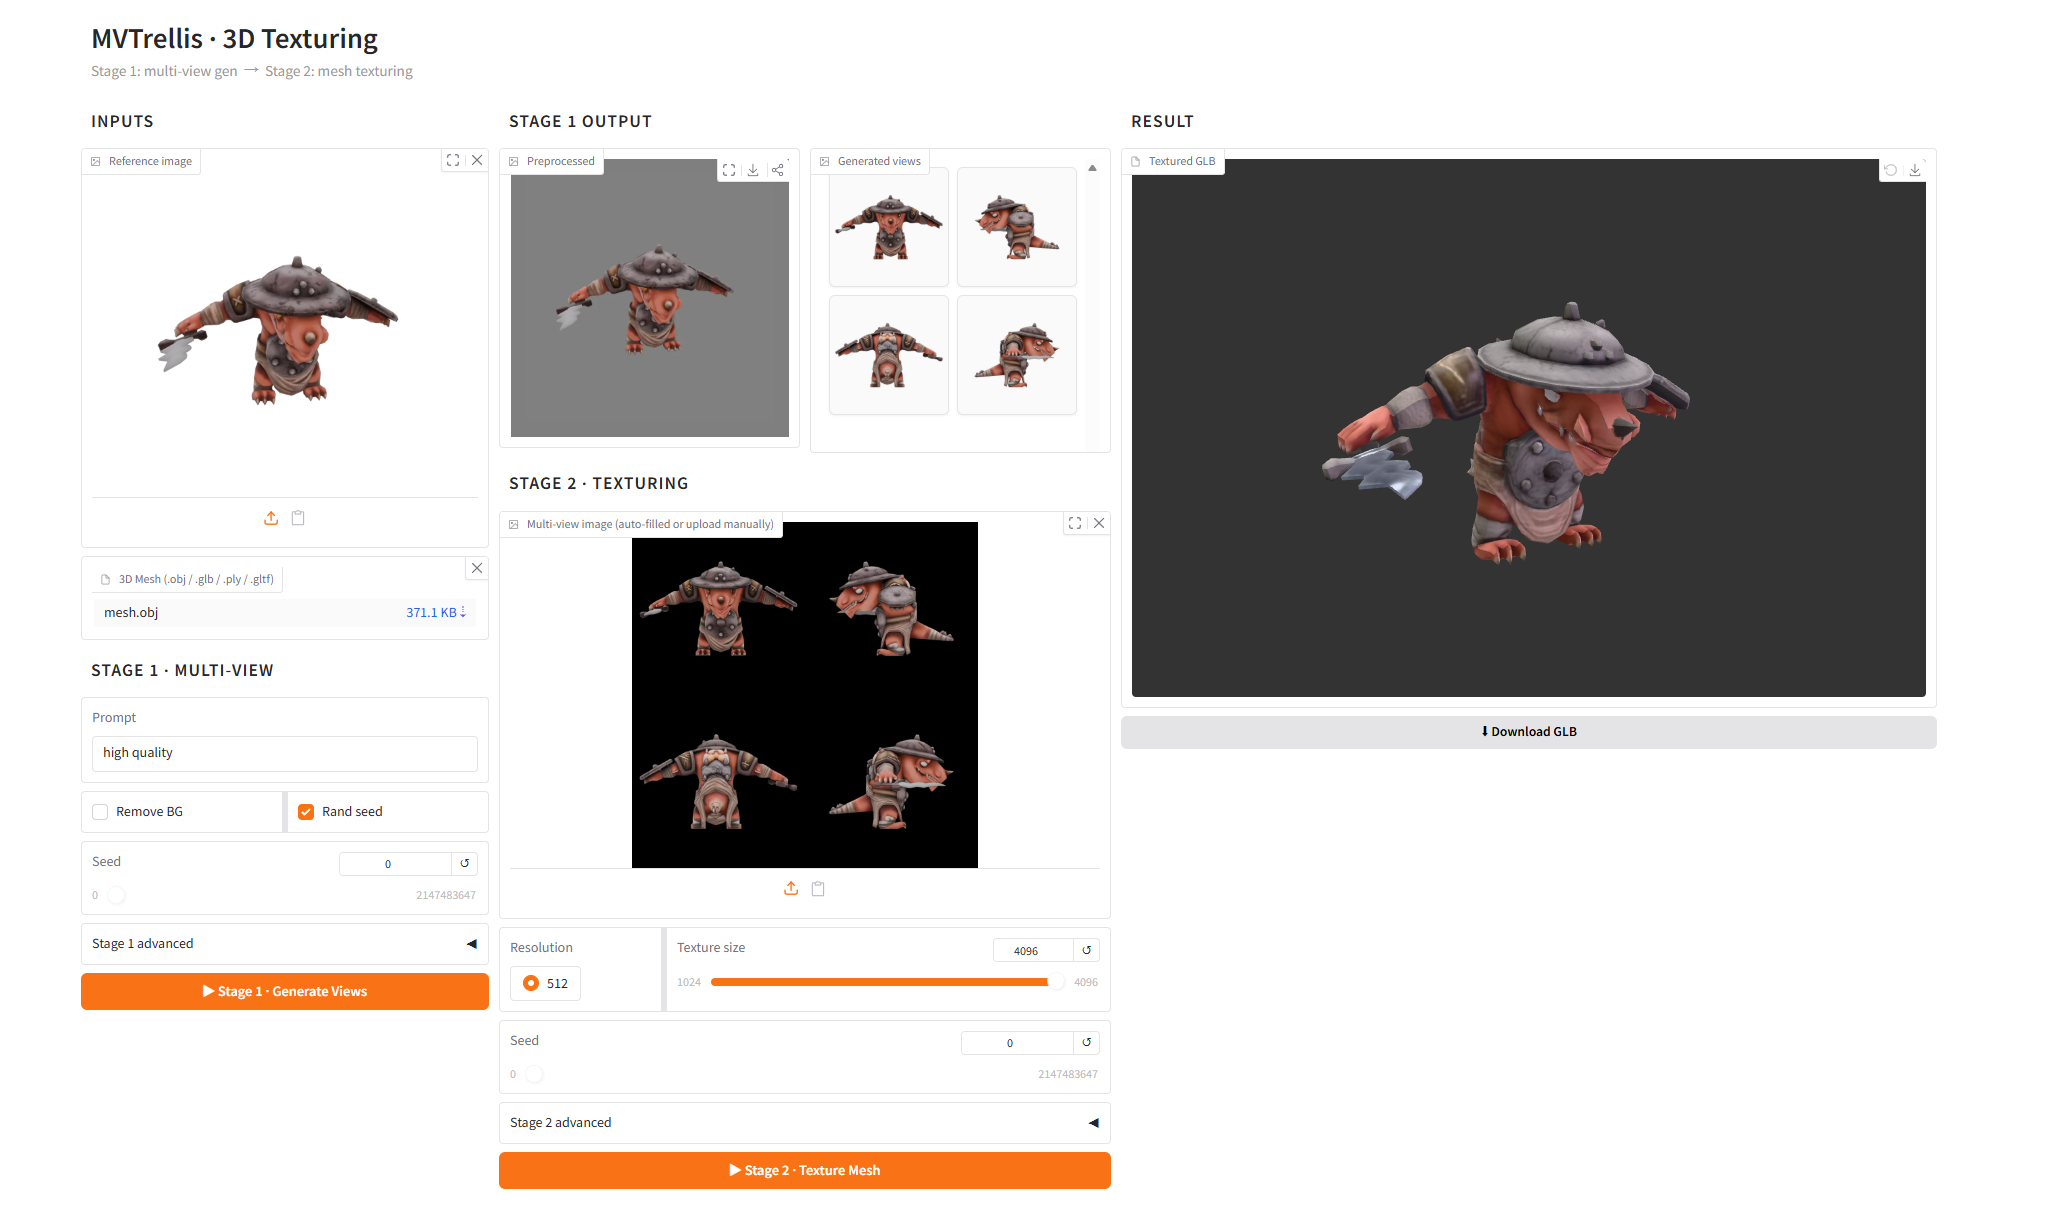
\includegraphics[width=\linewidth]{figure/final/user.png}
    \caption{
        系统用户界面。界面采用三栏布局，
        从左至右依次为输入与第一阶段参数控制区、
        多视角生成结果与第二阶段参数控制区、
        以及最终纹理化三维模型交互预览区。
        上图展示了以单张正面参考图为条件，
        经两阶段生成后所得纹理化三维模型的完整操作流程。
    }
    \label{fig:user}
\end{figure}

左栏为输入区域（Inputs）与第一阶段参数控制区（Stage 1 · Multi-View）。
用户在此上传裸网格文件（支持 .obj、.glb、.ply、.gltf 格式）
与单张参考图像，并可配置提示词、是否执行背景去除、
随机种子及 CFG 引导强度等参数，
点击“Stage 1 · Generate Views”按钮触发多视角图像生成。

中栏分为上下两部分。
上半部分为第一阶段输出区（Stage 1 Output），
并排展示经预处理的参考图像与生成的四视角图像，
供用户直观评估多视角外观的一致性与风格符合程度。
下半部分为第二阶段控制区（Stage 2 · Texturing），
展示自动拼接生成的 $2\times2$ 多视图拼图，
该拼图同时作为 Trellis.2 的条件输入，
用户亦可手动上传自定义多视图图像以替换自动结果，
并配置纹理分辨率、采样步数等参数后
点击“Stage 2 · Texture Mesh”触发三维纹理生成。

右栏为结果展示区（Result），
内嵌交互式三维模型查看器，
支持旋转、缩放与平移操作，
可实时预览最终纹理化三维模型，
并提供 GLB 格式文件下载。



